\documentclass[conference]{IEEEtran}
\IEEEoverridecommandlockouts
% The preceding line is only needed to identify funding in the first footnote. If that is unneeded, please comment it out.
\usepackage{cite}
\usepackage{amsmath,amssymb,amsfonts}
\usepackage{algorithmic}
\usepackage{graphicx}
\usepackage{textcomp}
\usepackage{xcolor}
\graphicspath{{./Screenshots}}

\def\BibTeX{{\rm B\kern-.05em{\sc i\kern-.025em b}\kern-.08em
    T\kern-.1667em\lower.7ex\hbox{E}\kern-.125emX}}
\begin{document}

\title{Towards Robust Federated Learning using Knowledge Distillation Techniques\\}

\author{\IEEEauthorblockN{Arindam Jain}
\IEEEauthorblockA{School of Computing \& Augmented Intelligence \\
Arizona State University \\
ajain243@asu.edu}
\and
\IEEEauthorblockN{Kiran Sthanusubramonian}
\IEEEauthorblockA{School of Computing \& Augmented Intelligence \\
Arizona State University \\
ksthanus@asu.edu}
}

\maketitle

\section{Introduction}
With the onset of improved privacy standards, edge computing capabilities, and large-scale machine learning requirements, Federated Learning has emerged as a privacy-preserving training paradigm for localized devices without data-sharing and aggregation requirements. With privacy-preserving benefits, users of these localized devices (e.g., mobile phones) also benefit from lower latencies in terms of required responses. Potential Federated Learning applications include improved mobile computing \cite{b1}, healthcare \cite{b2}, and autonomous vehicles. \\
In this project, we explore the use of Knowledge Distillation (KD) to create highly accurate and robust Federated Learning paradigms. Knowledge Distillation is conceptualized as a model compression technique in which large models with complex architectures are used to train a single smaller model that can run on devices with lesser computational capabilities while still achieving comparable performance levels. The most common Knowledge Distillation architecture is the Teacher-Student architecture (Fig.1). \\
The rest of this proposal is arranged as follows: Section II will detail the findings of the Literature Survey (including potential shortcomings), Section III will highlight the Problem Statement, Section IV will discuss the Methodology (including execution plan, datasets to be used, and the metrics to evaluate \& validate the methodology), Section V will summarize the objectives and learning outcomes from this project.
\begin{figure}[htbp]
\centering
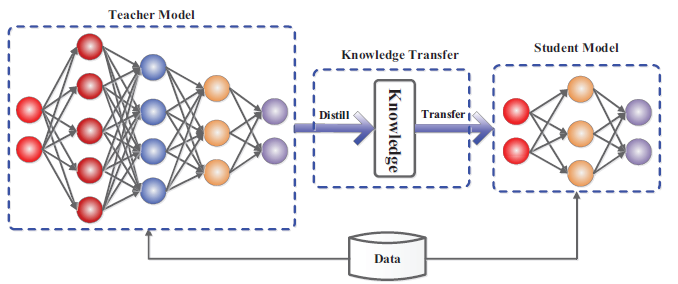
\includegraphics[scale=0.5]{Knowledge_Distillation.png}
\caption{Teacher-Student Architecture for Knowledge Distillation \cite{b3}}
\label{fig}
\end{figure}
\section{Literature Survey}
\subsection{Knowledge Distillation Techniques for Federated Learning}
One of the popular KD Algorithms for Heterogenous Federated Learning is proposed as FedMD (Li \& Wang) \cite{b4}. Here, the primary assumption is that our local nodes have the computation capability of defining and training their NN models specific to their local datasets - this helps solve the statistical heterogeneity of data across the nodes. FedMD focuses on utilizing the core idea of KD, i.e., using the Prediction Logits output from local Neural Network (NN) models averaged out as Knowledge to reach a better global consensus. FedMD also employs Knowledge Transfer (using a single large global dataset) to overcome the issue of small local datasets. However, this paradigm is prone to Byzantine Faults and potential corruption of the global consensus due to adversarial attacks on one or more of the local nodes. Furthermore, the communication efficiency of the overall network architecture reduces as the number of nodes increases. \\

Related work to Robust Federated Learning is done in \cite{b5}, where several Client (Teacher) models are fused into a single Server (Student) model, which is further trained using unlabeled datasets to improve robustness. However, this does not defend against potential adversaries (a similar drawback to the algorithm presented in FedMD).
\subsection{Improving Fairness and Robustness of Federated Learning Architectures}
To improve the fairness, accuracy, and robustness of Federated Learning architectures to potential Byzantine faults and adversarial attacks, we take inspiration from the algorithm proposed in Ditto (Tian Li et al) \cite{b6}. Here, personalization is used as a technique to balance robustness and fairness requirements. Personalization is mathematically conceptualized through regularization during local model updation with the global consensus calculated. The regularized parameter is tuned with respect to several factors, such as local dataset sample size, number of nodes affected by adversarial attacks, etc.
\section{Problem Statement}

\section{Methodology}
\subsection{Execution Plan}
\subsection{Datasets}
\subsection{Evaluation Metrics}

\section{Objectives \& Learning Outcomes}

\begin{table}[htbp]
\caption{Table Type Styles}
\begin{center}
\begin{tabular}{|c|c|c|c|}
\hline
\textbf{Table}&\multicolumn{3}{|c|}{\textbf{Table Column Head}} \\
\cline{2-4} 
\textbf{Head} & \textbf{\textit{Table column subhead}}& \textbf{\textit{Subhead}}& \textbf{\textit{Subhead}} \\
\hline
copy& More table copy$^{\mathrm{a}}$& &  \\
\hline
\multicolumn{4}{l}{$^{\mathrm{a}}$Sample of a Table footnote.}
\end{tabular}
\label{tab1}
\end{center}
\end{table}

\begin{thebibliography}{00}
\bibitem{b1} W. Y. B. Lim et al., "Federated Learning in Mobile Edge Networks: A Comprehensive Survey," in IEEE Communications Surveys \& Tutorials, vol. 22, no. 3, pp. 2031-2063, third quarter 2020.
\bibitem{b2} Xu, J., Glicksberg, B.S., Su, C. et al. Federated Learning for Healthcare Informatics. J Healthc Inform Res 5, 1–19 (2021).
\bibitem{b3} Gou, J., Yu, B., Maybank, S.J. et al. Knowledge Distillation: A Survey. Int J Comput Vis 129, 1789–1819 (2021).
\bibitem{b4} Li, Daliang and Junpu Wang. “FedMD: Heterogenous Federated Learning via Model Distillation.” ArXiv abs/1910.03581 (2019)
\bibitem{b5} Tao Lin, Lingjing Kong, Sebastian U. Stich, and Martin Jaggi. 2020. Ensemble distillation for robust model fusion in federated learning. In Proceedings of the 34th International Conference on Neural Information Processing Systems (NIPS'20). Curran Associates Inc., Red Hook, NY, USA, Article 198, 2351–2363.
\bibitem{b6} Tian Li, Shengyuan Hu, Ahmad Beirami \& Virginia Smith. (2021). Ditto: Fair and Robust Federated Learning Through Personalization. 
\end{thebibliography}

\end{document}